% SI Text 6: strategic timing of funding. Moved from the main text's Results on 2026-09-29
% (revision plan 2, Package B). The text is the former Results subsection with three stated
% limits added; the figure is the former main-text Fig. 4. Terms: "the forward-looking
% funder's timing" (not "optimal timing"); ``gain from planning ahead'' (not "timing gain").
\section{Strategic timing of funding}\label{si:timing}
The funder holds a fixed budget for the whole horizon and may time its spending freely. The strongest argument for spending early concerns fields whose researchers have few resources: a researcher without resources produces nothing, so the funder observes nothing and no capability grows, and money held for later rounds produces neither evidence nor growth in the meantime. The argument fails. A funder that spends everything in the first round allocates before observing any research output, and knows exactly as little as a funder that spends everything in the last round; in a field with no resources at all, the two produce identical expected output. What the argument does establish is a complementarity: early spending enables observation and growth, and late spending exploits what early spending revealed. That favors putting some money early. It does not favor putting most of it early.

In our simulations, under complementarity, observation comes first and money second. Wherever capabilities compound at more than a negligible rate ($\epsilon$ above about 0.03), the forward-looking funder spends less than an even share in the first round and spends the bulk once output has revealed who is capable; scarce baseline resources raise the early share and weaken the effect, but do not reverse it (Fig.~\ref{fig:p3}\textit{A}). The shift of spending toward later rounds comes from the output researchers produce whether or not they are funded, which compounds and reveals capability while the funder waits (\ref{si:extended}, Fig.~\ref{fig:depth-schedule}).

Planning ahead is worth less than the signal provided by grant peer review, in every setting we test. Across all horizons and compounding rates in our sweeps, the forward-looking funder's gain over the myopic funder, which spends equal installments each round, stays below the review signal's value: by an order of magnitude or more at the default compounding rate and below, and approaching the signal's value only at the highest compounding rate and the longest horizon we consider (Fig.~\ref{fig:p3}\textit{B}). As a share of the research output that the forward-looking funder's funding adds, the gain from planning ahead ranges from indistinguishable from zero to 4.5\% across the 30 settings tested; the review signal's value in the same settings ranges from 7\% to 27\%. The gain exists only where capability and resources are complements: under Cobb-Douglas production it is indistinguishable from zero (\ref{app:technology}, Table~\ref{tab:timing-technology}).

Three limits bound these results, and they are the reason the timing analysis sits in the SI rather than the main text. First, the forward-looking funder is a certainty-equivalent planner (SI Materials and Methods): it treats future output as equal to its expectation and does not value the information its own grants will generate, so it is not the Bayes-optimal sequential policy, and its gain is a lower bound on what planning ahead could be worth. Second, the gain combines two changes at once, when the money is spent and whom it reaches, because a funder that anticipates capability growth also values recipients differently; we do not separate the two, and ``gain from planning ahead'' names their sum. Third, the objective counts output within the horizon only and assigns no value to the capability that remains at its end. A terminal value for capability would credit the capability that late grants build, which the horizon objective ignores, and also the compounded capability that early grants leave behind; we have not measured which effect is larger, so the size of the shift toward later rounds should be read as specific to the horizon objective.

\begin{figure}[tp]
\centering
\begin{minipage}{\linewidth}\noindent\textbf{A}\par\vspace{-0.3em}
\begin{tikzpicture}
\begin{axis}[
  width=0.79\linewidth, height=5.4cm,
  axis lines*=left,
  xmode=log,
  xmin=0.0001, xmax=0.85, ymin=0.48, ymax=0.68,
  xtick={0.0001, 0.01, 0.1, 0.85},
  xticklabels={0.0001, 0.01, 0.1, 0.85},
  ytick={0.5, 0.55, 0.6, 0.65},
  yticklabels={even, 0.55, 0.60, 0.65},
  xlabel={compounding rate $\epsilon$},
  ylabel={center of mass of spending},
  ylabel style={font=\small}, xlabel style={font=\small},
  tick label style={font=\small},
  axis line style={line width=0.4pt},
  tick style={line width=0.4pt, black},
  clip=false,
]
\addplot[gray, dashed, line width=0.4pt, domain=0.0001:0.85] {0.5};
\addplot[black, line width=0.7pt] table[x=eps, y=rich] {fig8-boundary.dat};
\addplot[black, line width=0.7pt] table[x=eps, y=mid]  {fig8-boundary.dat};
\addplot[black, line width=0.7pt] table[x=eps, y=poor] {fig8-boundary.dat};
\node[font=\small, anchor=west] at (axis cs:0.92,0.652) {many resources};
\node[font=\small, anchor=west] at (axis cs:0.92,0.566) {intermediate};
\node[font=\small, anchor=west] at (axis cs:0.92,0.521) {few resources};
\end{axis}
\end{tikzpicture}
\end{minipage}\par\vspace{0.9em}
\begin{minipage}{\linewidth}\noindent\textbf{B}\par\vspace{-0.3em}
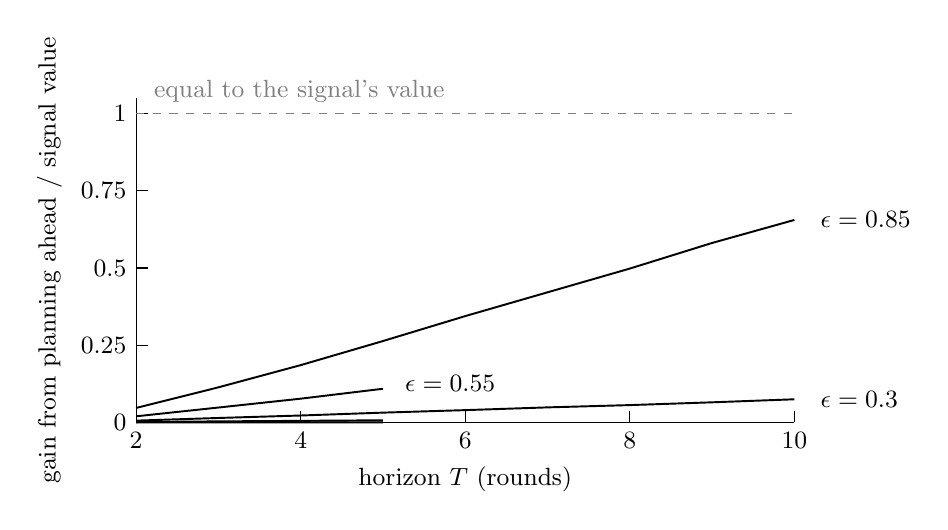
\begin{tikzpicture}
\begin{axis}[
  width=0.82\linewidth, height=5.7cm,
  axis lines*=left,
  xmin=2, xmax=10, ymin=0, ymax=1.05,
  xtick={2, 4, 6, 8, 10},
  ytick={0, 0.25, 0.5, 0.75, 1},
  yticklabels={0, 0.25, 0.5, 0.75, 1},
  xlabel={horizon $T$ (rounds)},
  ylabel={gain from planning ahead / signal value},
  ylabel style={font=\small}, xlabel style={font=\small},
  tick label style={font=\small},
  axis line style={line width=0.4pt},
  tick style={line width=0.4pt, black},
  clip=false,
]
\addplot[gray, dashed, line width=0.4pt, domain=2:10] {1};
\node[font=\small, gray, anchor=south west] at (axis cs:2.1,1.005) {equal to the signal's value};
\addplot[black, line width=0.7pt] coordinates {(2,0.0468) (3,0.1136) (4,0.1855) (5,0.2635) (6,0.3443) (7,0.4213) (8,0.4982) (9,0.5811) (10,0.6556)};
\addplot[black, line width=0.7pt] coordinates {(2,0.0198) (3,0.0482) (4,0.0769) (5,0.1090)};
\addplot[black, line width=0.7pt] coordinates {(2,0.0058) (3,0.0144) (4,0.0224) (5,0.0317) (6,0.0398) (7,0.0487) (8,0.0561) (9,0.0651) (10,0.0749)};
\addplot[black, line width=0.7pt] coordinates {(2,0.0012) (3,0.0034) (4,0.0051) (5,0.0069)};
\addplot[black, line width=0.7pt] coordinates {(2,0.0000) (3,0.0002) (4,0.0001) (5,0.0000)};
\node[font=\small, anchor=west] at (axis cs:10.2,0.656) {$\epsilon = 0.85$};
\node[font=\small, anchor=west] at (axis cs:5.15,0.126) {$\epsilon = 0.55$};
\node[font=\small, anchor=west] at (axis cs:10.2,0.075) {$\epsilon = 0.3$};
\end{axis}
\end{tikzpicture}
\end{minipage}\par\vspace{0.9em}
\caption{Strategic timing of funding. (\textit{A}) The compounding rate, not the scarcity of baseline resources, sets how far spending shifts toward later rounds: the center of mass of spending (0.5 is even; higher is later) as the compounding rate $\epsilon$ increases, for three baseline resource scales. (\textit{B}) Choosing whom outweighs choosing when: the gain from planning ahead, as a share of the review signal's value, by horizon and compounding rate; in every setting the gain is below the signal's value. Settings: SI Materials and Methods.}
\label{fig:p3}
\end{figure}

